\begin{figure}[ht!]
\centering
\subfigure{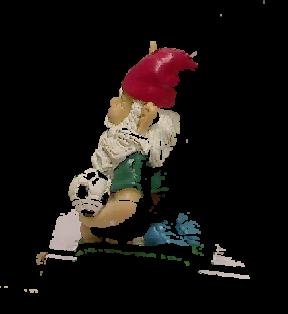
\includegraphics[width=.45\linewidth]{figures/results/100deg}}\quad
\subfigure{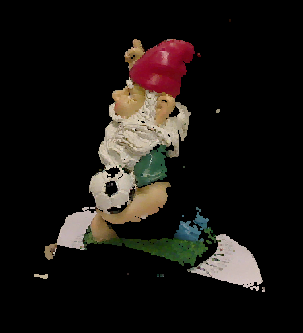
\includegraphics[width=.45\linewidth]{figures/results/80deg}}\\
\subfigure{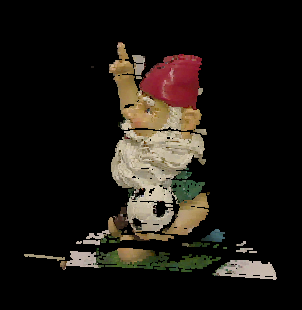
\includegraphics[width=.45\linewidth]{figures/results/60deg}}\quad
\subfigure{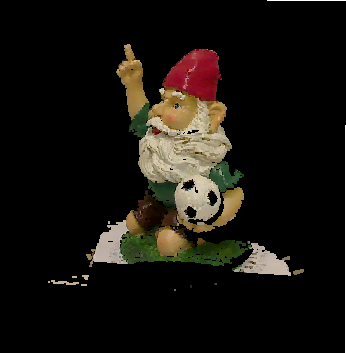
\includegraphics[width=.45\linewidth]{figures/results/40deg}}\\
\subfigure{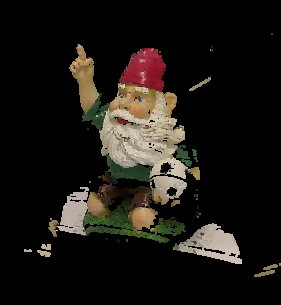
\includegraphics[width=.45\linewidth]{figures/results/20deg}}\quad
\subfigure{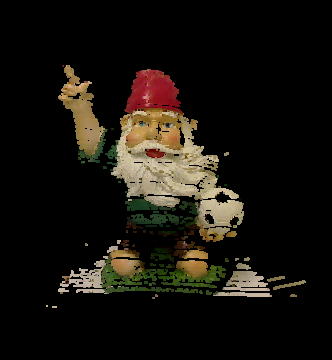
\includegraphics[width=.45\linewidth]{figures/results/0deg}}\\
\caption{Results}
\label{figure:results}
\end{figure}

The imaging system in addition to the source directory, expects a reference
image without the laser stripe and two images of the individual background
patterns used for calibration as input. The program saves the point cloud thus
obtained in a destination directory which is used by the \ac{3DTK} components
for processing and visualization. The results obtained from the
\texttt{show} program are shown in Fig. \ref{figure:results}.
